%\documentclass{beamer}
%\documentclass[c]{beamer}
 \documentclass[t]{beamer}
%\documentclass[b]{beamer}
\listfiles

\mode<presentation>
{
  \usetheme[english]{KIT}
% \usetheme[usefoot]{KIT}
% \usetheme[deutsch]{KIT}

%%  \usefonttheme{structurebold}

  \setbeamercovered{transparent}

  %\setbeamertemplate{enumerate items}[circle]
  \setbeamertemplate{enumerate items}[ball]
}

\usepackage{babel}
\date{29.10.13}
%\DateText

%\KITfoot{\parbox[t]{90mm}{\today:\qquad Dies ist eine sehr lange selbstdefinierte Fu\ss{}zeile -- Dies ist eine sehr lange selbstdefinierte Fu\ss{}zeile -- Dies ist eine sehr lange selbstdefinierte Fu\ss{}zeile}}


\usepackage[utf8]{inputenc}
\usepackage[T1]{fontenc}
\usepackage{array}
\usepackage{minted}

\usenavigationsymbols
%\usenavigationsymbols[sfHhdb]
%\usenavigationsymbols[sfhHb]

%\title[Python Interfaces for reactor codes]{Python Interfaces for Reactor Codes}
\title[Python framework for coupled reactor calculations]{PIRS: Python-based Framework for coupled MC-TH Reactor Calculations}
\subtitle{SNA-MC 2013}

\author{A.Travleev, R. Molitor, V.H. Sanchez}
%\author{А. Травлеев, Р. Молитор, В. Санчез}

%\institute{Карлсруйский технологический институт, институт физики нейтронов и техники реакторов}
\institute{Institute for Neutron Physics and Reactor Technology}

%\TitleImage[height=\titleimageht]{Bilder/bildwand.jpg}
\TitleImage[height=\titleimageht]{Bilder/KIT-Titel.png}


\begin{document}

\begin{frame}
  \maketitle
\end{frame}

\begin{frame}\frametitle{Content}

    \begin{itemize}
        \item Introduction: what is PIRS, example

        \item PIRS concept

        \item Current development status

        \item Outlook

    \end{itemize}
\end{frame}

\section{Introduction}
\begin{frame}\frametitle{What is PIRS}

    \begin{block}{PIRS: Python Interfaces for Reactor Simulations}

    A set of packages for Python programming language, to facilitate
    interaction with reactor calculation codes.
    \end{block}

    \begin{columns}
        \column{0.45\textwidth}
    \begin{block}{Python}
    \begin{itemize}

        \item www.python.org

        \item Free 

        \item Interpreted

        \item OS-independent

        \item Big community

        \item Lot of packages 

    \end{itemize}
    \end{block}

        \column{0.45\textwidth}
    \begin{block}{Interaction with code}
    \begin{itemize}
        
        \item Model description

        \item Generation of Input file(s)

        \item Job submission

        \item Reading of calculation results

    \end{itemize}
    \end{block}
    \end{columns}
\end{frame}

\begin{frame}\frametitle{What for?}    

    
    \begin{itemize}
    \item Routine preparation of input files 

    \item Framework for coupled calculations

    \item ...
    \end{itemize}

\end{frame}

\newcommand{\exModel}{Example: simplified neutronics model of fuel pin}
\begin{frame}[fragile]
    \frametitle{\exModel}

    Geometry:
    \inputminted[frame=single,fontfamily=tt,fontsize=\footnotesize]{python}{geom.py}

\end{frame}

\begin{frame}[fragile]
    \frametitle{\exModel}

    Neutronics:

    \begin{columns}
        \column{0.45\textwidth}
            \inputminted[frame=single,fontfamily=tt,fontsize=\footnotesize,firstline=3,lastline=17]{python}{mc_int.py}
        \column{0.45\textwidth}
            \inputminted[frame=single,fontfamily=tt,fontsize=\footnotesize,firstline=17]{python}{mc_int.py}
    \end{columns}

\end{frame}

\begin{frame}[fragile,plain]
    \frametitle{\exModel}
    \begin{columns}
        \column{0.45\textwidth}
            {\tiny Generated MCNP input file}
            \inputminted[frame=single,fontfamily=tt,fontsize=\tiny,firstline=3,lastline=33]{rst}{mcnp0/i_}
        \column{0.45\textwidth}
            \inputminted[frame=single,fontfamily=tt,fontsize=\tiny,firstline=34]{rst}{mcnp0/i_}
    \end{columns}
\end{frame}

\begin{frame}[fragile]
    \frametitle{\exModel}

    {\small Geometry plot generated with MCNP}
    \includegraphics[width=0.7\textwidth]{mcnp0/i__p02.pdf}
\end{frame}

\section{Concept}
\begin{frame}\frametitle{Concept}
    \begin{block}{Class types}
        \begin{itemize}
            \item To describe calculation geometry:
                  Solids (Cylinder, Box) can be inserted into each other and
                  positioned with respect to container.

            \item Low-level interfaces:
                \begin{itemize}
                    \item Assure correct syntax of input file, 
                    \item "Know" command line parameters of the code, 
                    \item provide functions to read output. 
                \end{itemize}

            \item High-level interfaces:
                \begin{itemize}
                    \item Conversion: geometry $\Longleftrightarrow$ low-level interfaces,
                    \item Interface to specify code-specific parameters
                \end{itemize}
        \end{itemize}
    \end{block}

%     \begin{block}{Users}
%         \begin{itemize}
%             \item расчетчики: используют геометрические классы и классы высокого уровня
%             \item разработчики интерфейсов: пишут интерфейсы
%         \end{itemize}
%     \end{block}
\end{frame}
\begin{frame}\frametitle{Concept}
   
    \begin{columns}
        \column{0.7\textwidth}
            \begin{block}{Interaction between classes}
            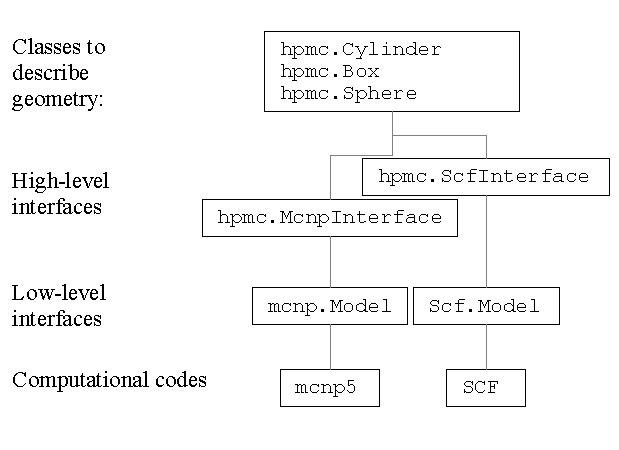
\includegraphics[width=\textwidth]{pics/scheme_en.pdf}
            \end{block}
        \column{0.3\textwidth}{\small
                \begin{block}{Geometry classes}
                    model dimensions, axial meshes for system variables (temperature, density, heat)
                \end{block}
                \begin{block}{High-level interfaces}
                    code-specific data, e.g. path to xsdir, isotopic material compositions for MCNP
                \end{block}
    }\end{columns}

\end{frame}

\section{Current development status}
\begin{frame}\frametitle{Current development status}
    Governed by HPMC project: Monte-Carlo neutronics and sub-channel TH modelling of PWR assembly.

    
    \begin{columns}
    \column{0.47\textwidth}
    \begin{block}{Interface to MCNP}
        \begin{itemize}
            \item handles any geometry represented by boxes and cylinders
            \item Repeated structure can be modelled as lattice 
            \item Description of materials
                \begin{itemize}
                    \item Convenient definition of composition
                    \item Automatic choice of suffixes and interpolation of XS
                \end{itemize}
            \item Reading of meshtal
        \end{itemize}
    \end{block}

    \column{0.47\textwidth}
    \begin{block}{Means to set up geometry} 
        \begin{itemize}
            \item Cylinder: vertical cylinder of finite height
            \item Box: rectangular parallelepiped with facets perpendicular to axes
        \end{itemize}
    \end{block}
    \begin{block}{Interface to SCF}
        \begin{itemize}
            \item Only for PWR-like geometries
            \item Reading of output.txt
        \end{itemize}
    \end{block}
    \end{columns}

\end{frame}

\newcommand{\exResult}{Example: results for coupled MCNP-SCF calculations}
\begin{frame}\frametitle{\exResult}

    Coupled MCNP -- SCF calculations, organized with PIRS
    \begin{itemize}
        \item Model: PWR assembly 17x17,
        \item moderator channels,
        \item two different types of fuel pins,
        \item boron in coolant,
        \item Coolant-centered subchannels,
        \item non-uniform axial mesh,
        \item Calculations conducted on a linux desktop
        \item relaxation scheme for power axial distribution with varying relaxation parameter and increasing statistical precision

    \end{itemize}

\end{frame}

\begin{frame}\frametitle{\exResult}

    Horizontal cross-section of MCNP model:
    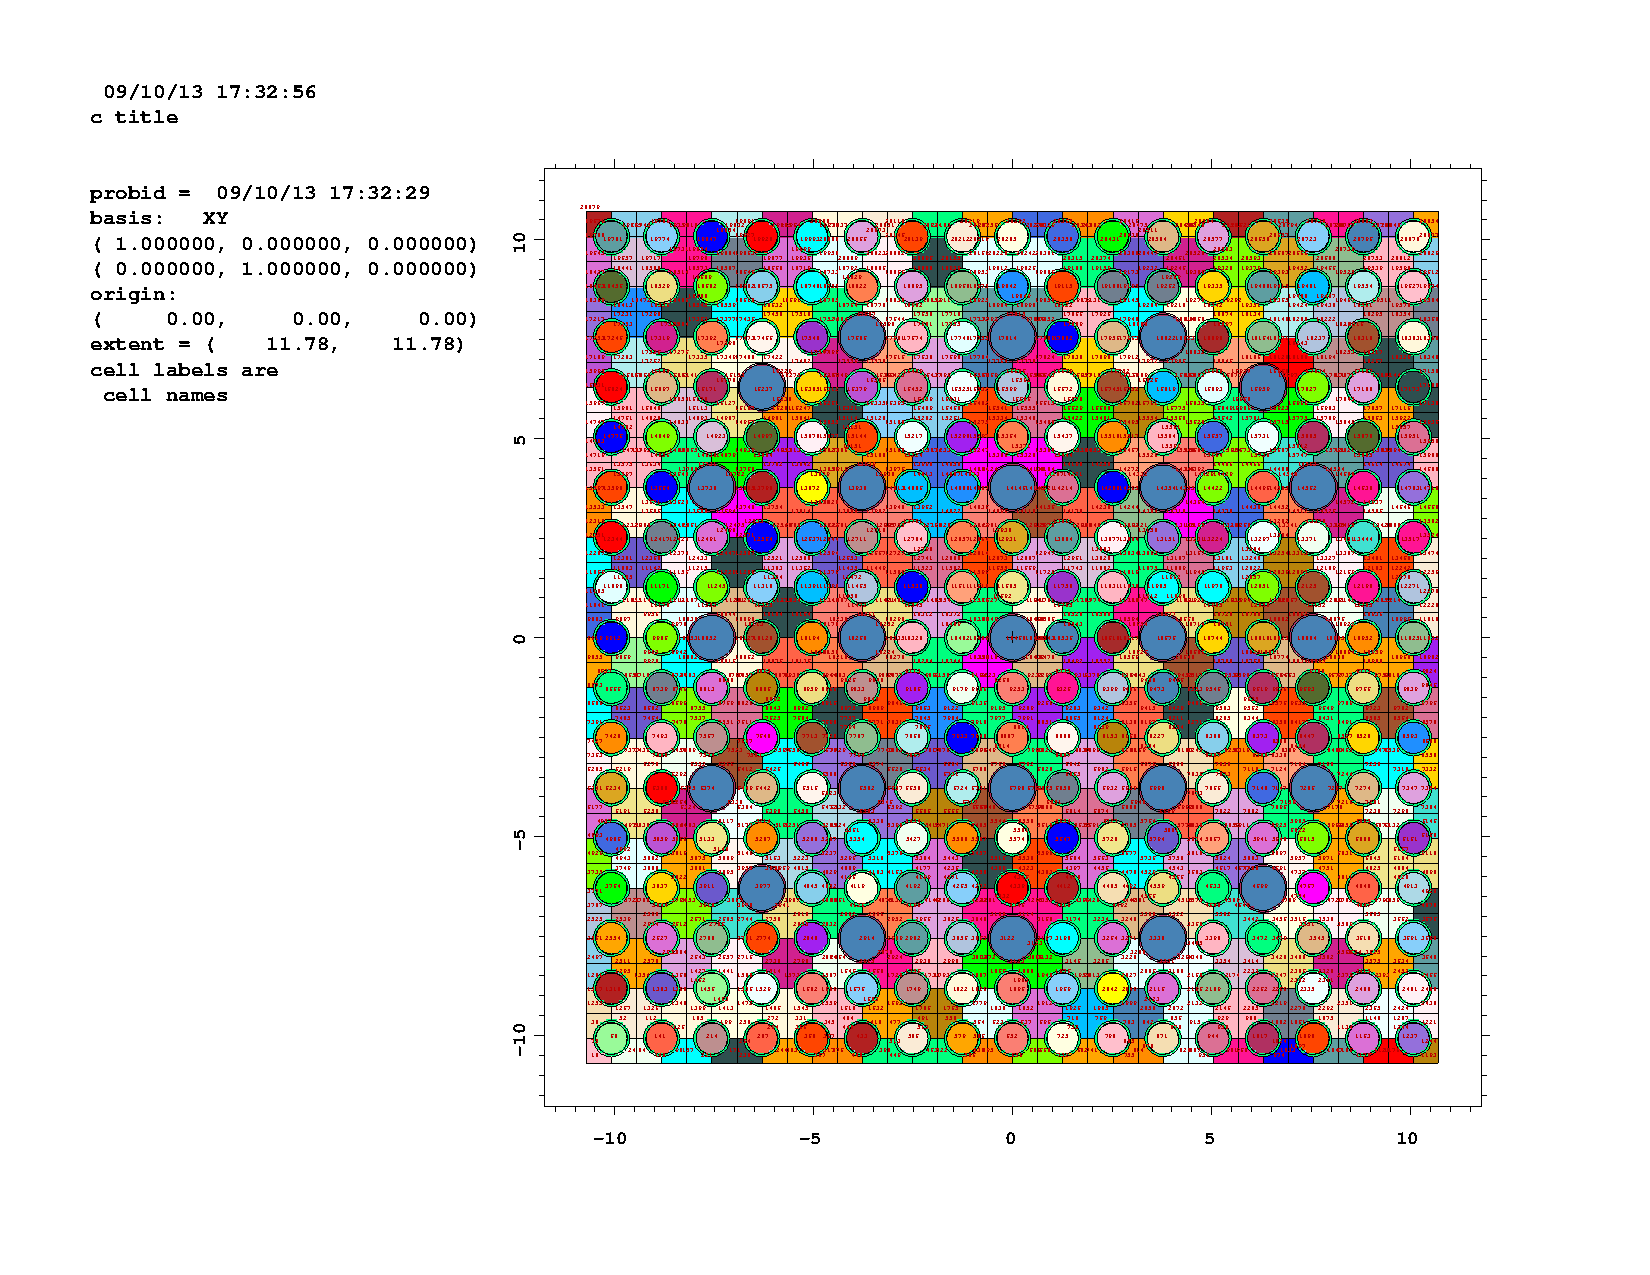
\includegraphics[width=0.7\textwidth]{pics/i__p01.pdf}

\end{frame}
\begin{frame}\frametitle{\exResult}

    Vertical cross-section of MCNP model:
    \includegraphics[width=0.7\textwidth]{pics/i__p02.pdf}

\end{frame}
\begin{frame}\frametitle{\exResult}

    Behaviour of  $k_{eff}$ with N--TH iterations 
    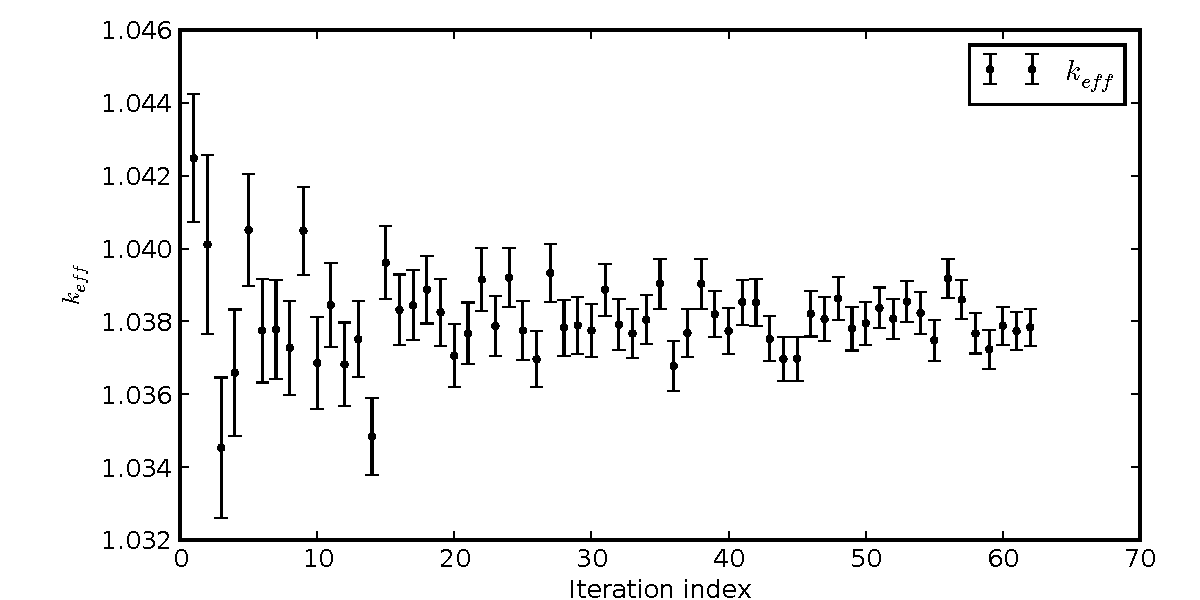
\includegraphics[width=0.8\textwidth]{pics/b_iteration_062_keff.pdf}
\end{frame}

\begin{frame}\frametitle{\exResult}
    Axial distribution of heat deposition in one fuel pin

    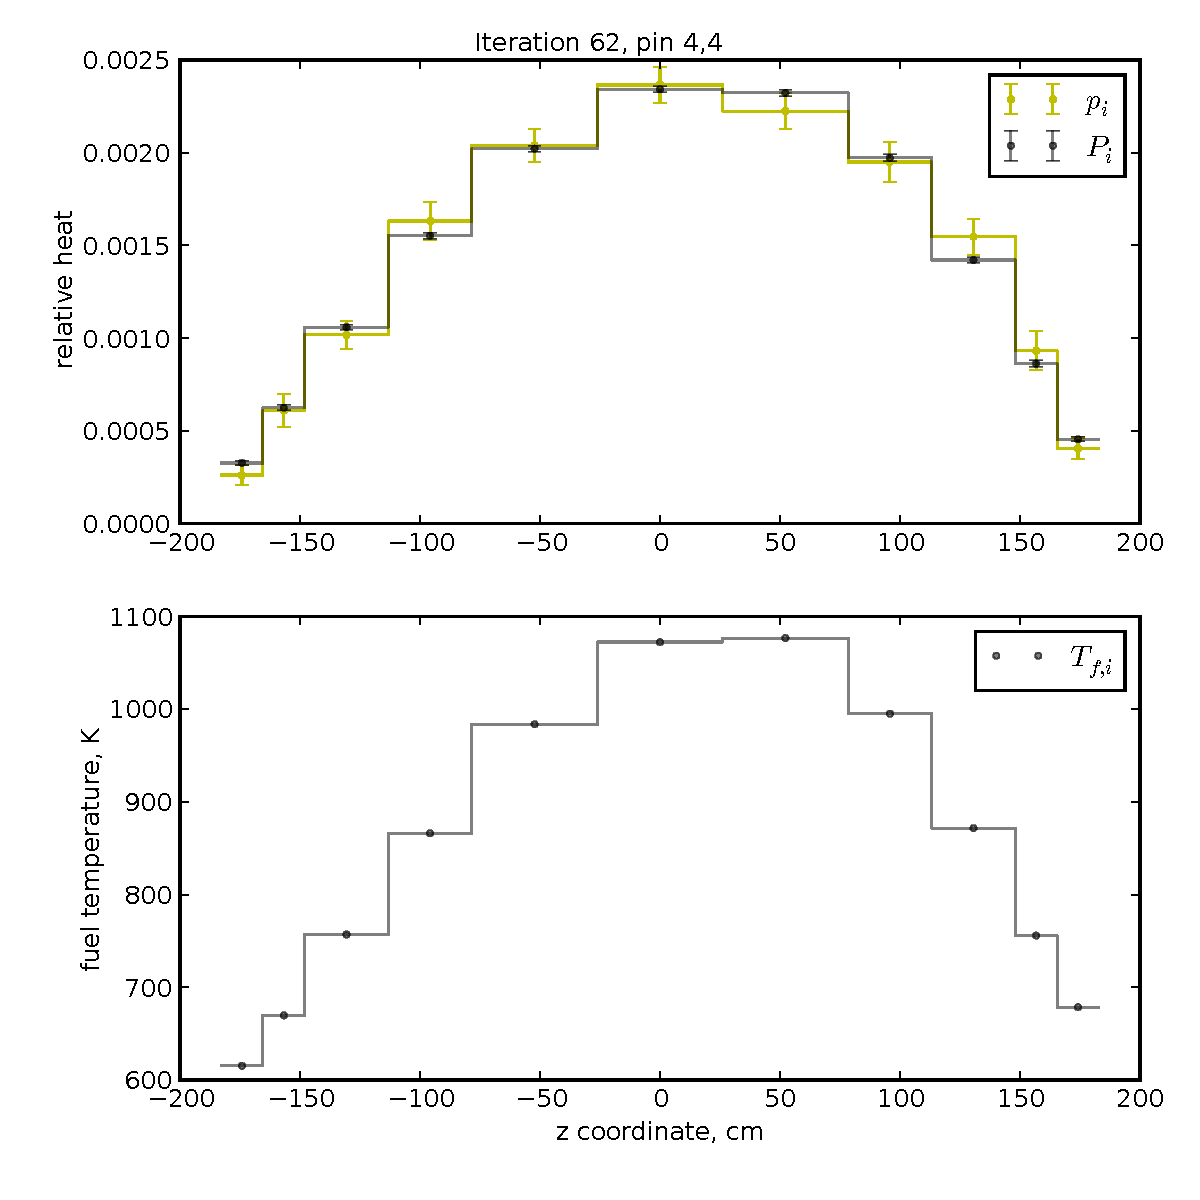
\includegraphics[trim=0 300 0 0,clip=true,width=0.8\textwidth]{pics/b_iteration_062_4_4.pdf}
\end{frame}

\begin{frame}\frametitle{\exResult}
    Axial distribution of fuel temperature in the same pin

    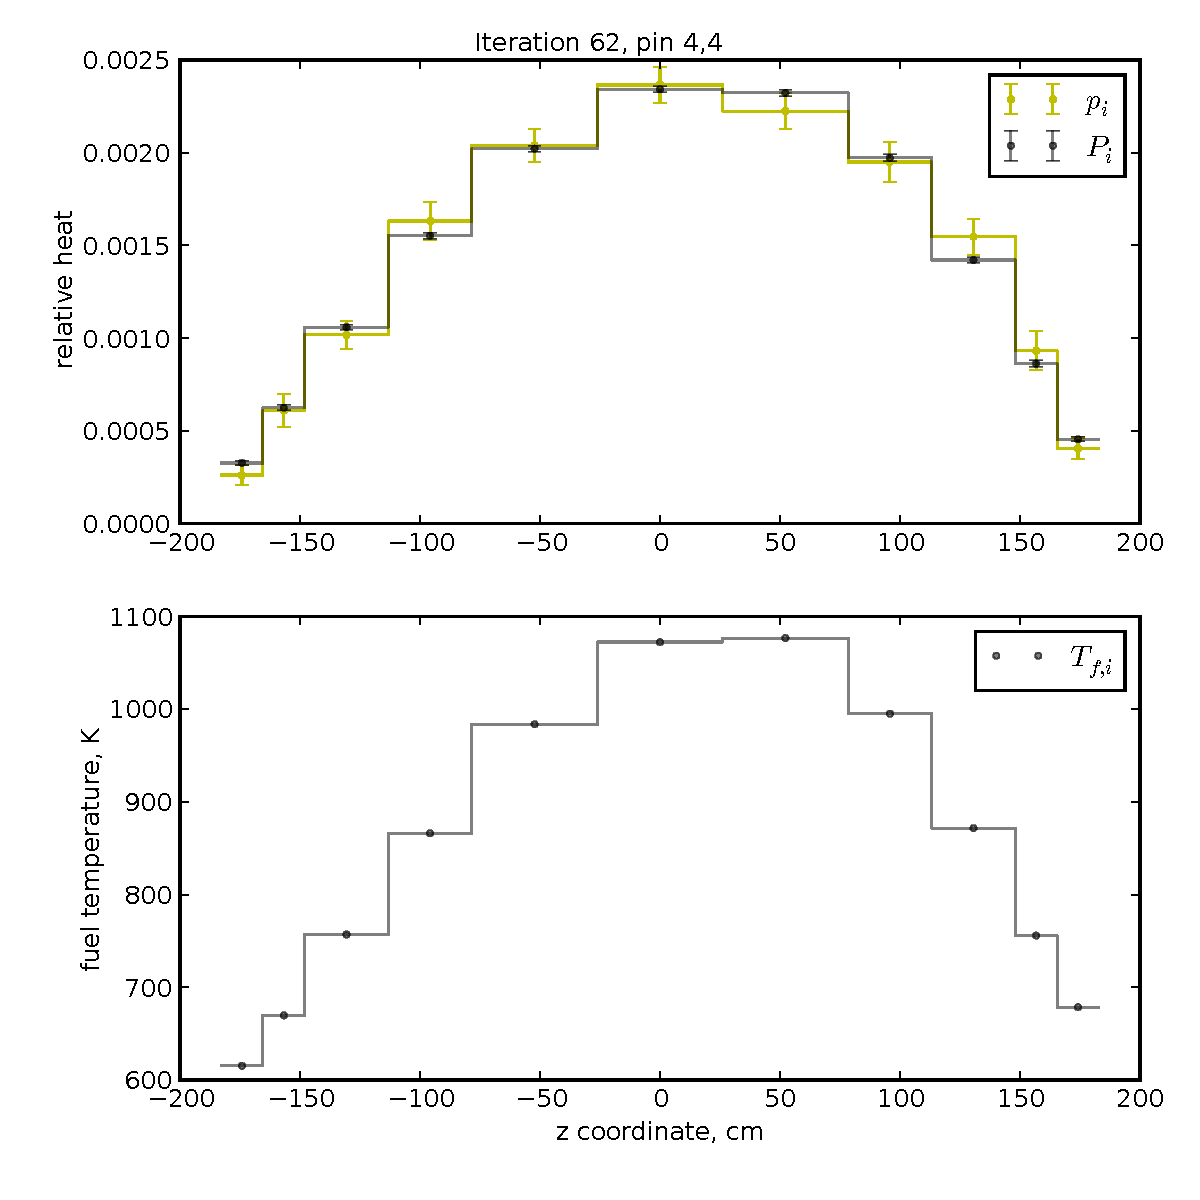
\includegraphics[trim=0 0 0 280,clip=true,width=0.8\textwidth]{pics/b_iteration_062_4_4.pdf}
\end{frame}

\begin{frame}\frametitle{\exResult}
    Temperature map

    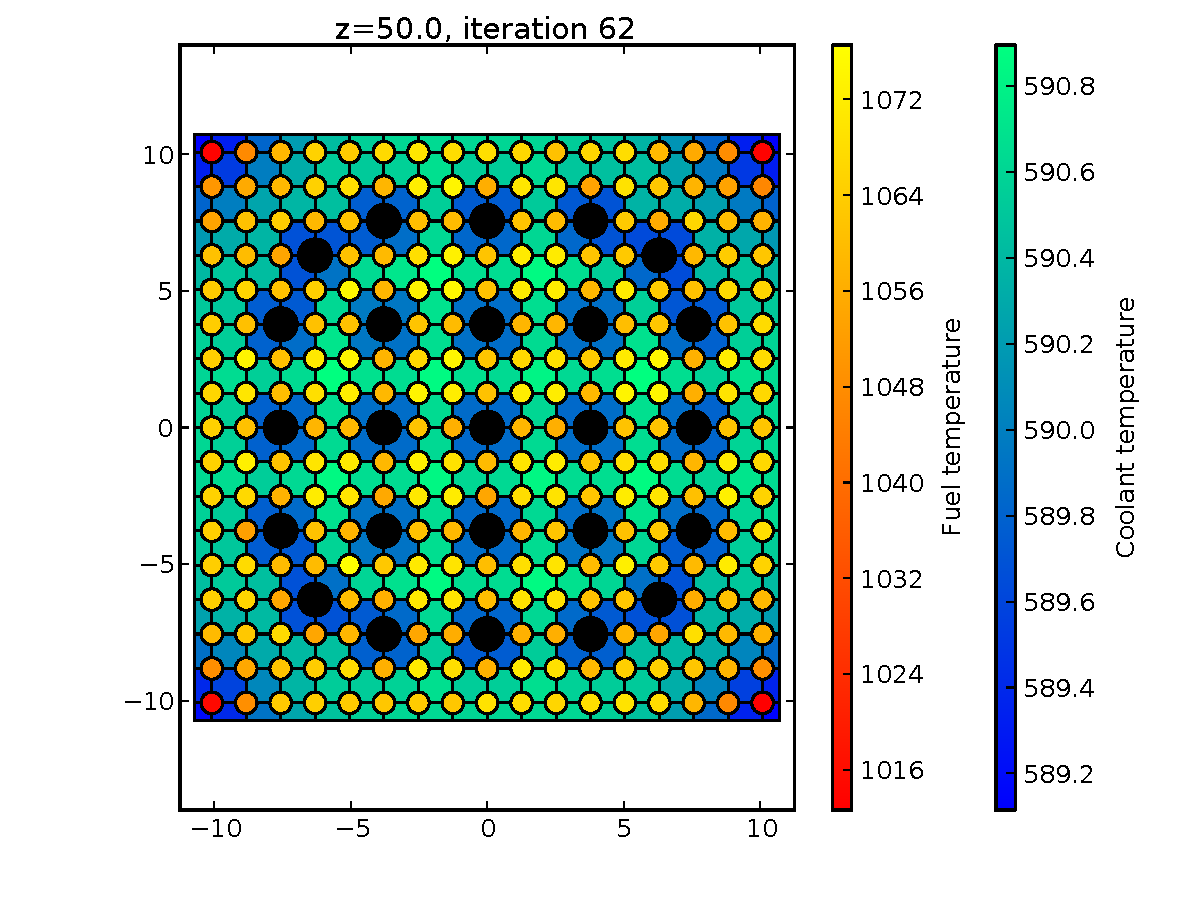
\includegraphics[width=0.7\textwidth]{pics/b_iteration_062_temp50_0.pdf}
\end{frame}


\section{Ongoing work}
\begin{frame}\frametitle{Ongoing work}

    \begin{block}{Curent}
        \begin{itemize}
            \item Interface to SERPENT-2
            \item Interaction with job submission system at Juelich Supercomputer
            \item Writing documentation
            \item Extension of SCF interface to represent cluster of assemblies, calculation of a minicore
        \end{itemize}
    \end{block}

    \begin{block}{Plans}
        \begin{itemize}
            \item New interface to SCF
            \item Geometry plotter
            \item Interface to NMC, parts of KANEXT
        \end{itemize}
    \end{block}

\end{frame}

\begin{frame}{Appendix}
\end{frame}

%\setbeamercolor{background canvas}{bg=violet}
\begin{frame}{Relaxation scheme}

    {\small
    Based on J.Dufek, W.Gudowski, "Stochastic Approximation for Monte Carlo
    Calculation of Steady-State Conditions in Thermal Reactors", {\it Nucl.
    Sci. Eng.}, Vol. 152, 2006, pp. 274.
    }

    \begin{columns}
        \column{0.5\textwidth}
            \fbox{
            
\includegraphics[page=2,viewport=105 120 500 450,clip=true,width=0.95\textwidth]{dufek.pdf}
            }
        \column{0.5\textwidth}
            \fbox{
            
\includegraphics[page=3,viewport=105 130 500 450,clip=true,width=0.95\textwidth]{dufek.pdf}
            }
    \end{columns}

\end{frame}

\end{document}
